% Copyright 2004 by Till Tantau <tantau@users.sourceforge.net>.
%
% In principle, this file can be redistributed and/or modified under
% the terms of the GNU Public License, version 2.
%
% However, this file is supposed to be a template to be modified
% for your own needs. For this reason, if you use this file as a
% template and not specifically distribute it as part of a another
% package/program, I grant the extra permission to freely copy and
% modify this file as you see fit and even to delete this copyright
% notice. 
% Adapted by Len Goff, 2019

\documentclass[10pt]{beamer}

% There are many different themes available for Beamer. A comprehensive
% list with examples is given here:
% http://deic.uab.es/~iblanes/beamer_gallery/index_by_theme.html
% You can uncomment the themes below if you would like to use a different
% one:
%\usetheme{AnnArbor}
%\usetheme{Antibes}
%\usetheme{Bergen}
%\usetheme{Berkeley}
%\usetheme{Berlin}
%\usetheme{Boadilla}
%\usetheme{boxes}
%\usetheme{CambridgeUS}
%\usetheme{Copenhagen}
%\usetheme{Darmstadt}
%\usetheme{default}
%\usetheme{Frankfurt}
%\usetheme{Goettingen}
%\usetheme{Hannover}
%\usetheme{Ilmenau}
%\usetheme{JuanLesPins}
%\usetheme{Luebeck}
\usetheme{Madrid}
%\usetheme{Malmoe}
%\usetheme{Marburg}
%\usetheme{Montpellier}
%\usetheme{PaloAlto}
%\usetheme{Pittsburgh}
%\usetheme{Rochester}
%\usetheme{Singapore}
%\usetheme{Szeged}
%\usetheme{Warsaw}

%Some code to format a hyperlink button
\setbeamertemplate{button}{\tikz[baseline={(0,-3.5pt)}]
	\node[
	inner xsep=5pt,
	inner ysep=1pt,
	draw=structure!80,
	fill=structure!50,
	rounded corners=4pt]  {\topskip0pt \normalsize\insertbuttontext};}

%Some packages that will be useful
\usepackage{pgfplots}
\usepackage{cancel}
\usepackage{caption}
\usepackage{dcolumn}
\usepackage{mathtools}
\captionsetup{belowskip=-15pt,aboveskip=0pt}

\usepackage{sansmathaccent}
\pdfmapfile{+sansmathaccent.map}

\usenavigationsymbolstemplate{}

\usepackage{array}
\newcolumntype{H}{>{\setbox0=\hbox\bgroup}c<{\egroup}@{}}
\usepackage{makecell}

\makeatletter
\def\thmhead@plain#1#2#3{%
	\thm@notefont{}% same as heading font
	\thmname{#1}\thmnumber{\@ifnotempty{#1}{ }\@upn{#2}}%
	\thmnote{ {\the\thm@notefont#3}}}
\let\thmhead\thmhead@plain
\itshape % body font
\makeatother

%Define normal density function for use in tikzpicture



%This allows adjustable spacing in itemize environment
\newenvironment{wideitemize}{\itemize\addtolength{\itemsep}{10pt}}{\enditemize}

%This allows slide numberering to not includethe title slide
\addtocounter{framenumber}{-1}
\addtobeamertemplate{navigation symbols}{}{%
	\usebeamerfont{footline}%
	\usebeamercolor[fg]{footline}%
	\hspace{1em}%
	%uncomment the below if you want frame numbers inside slide rather than in footline
	%\insertframenumber/\inserttotalframenumber
}

%
\newcommand{\backupbegin}{
	\newcounter{finalframe}
	\setcounter{finalframe}{\value{framenumber}}
}
\newcommand{\backupend}{
	\setcounter{framenumber}{\value{finalframe}}
}

\usetikzlibrary{decorations.pathreplacing,angles,quotes}
\usetikzlibrary{patterns}
\usetikzlibrary{positioning}
\usetikzlibrary{decorations.text}
\usetikzlibrary{decorations.pathmorphing}

%\title{Entangled instrumental variables}
\title{Theory-of-Languages-and-Machines}

% A subtitle is optional and this may be deleted
%\subtitle{Optional Subtitle}

\author{Shahla fathollahi}

\institute[Payam Noor university of Tehran] % (optional, but mostly needed)
{
	Introduction to Automata Theory,Formal Languages and Computation
	
	
                     Shyamalendu Kandar
}

\date{}

\usepackage{graphicx}
\usepackage{bbm}
%\definecolor{Gray}{gray}{0.85}
%\setbeamercolor{normal text}{fg=gray}
%\setbeamercolor{frametitle}{fg=green}
\graphicspath{ {images/} }
\setbeamercovered{}
\usepackage{tikz}
\usetikzlibrary{automata,positioning, arrows}
\usetikzlibrary{patterns, arrows}
\usetikzlibrary{arrows.meta,shapes.arrows}
%\usetikzlibrary{decorations.markings}
\tikzset{->, % makes the edges directed
>=stealth, % makes the arrow heads bold
node distance=3cm, % specifies the minimum distance between two nodes. Change if necessary.
every state/.style={thick, fill=gray!2}, % sets the properties for each ’state’ node
initial text=$ $, % sets the text that appears on the start arrow
}

\begin{document}

\begin{frame}
  \titlepage
\end{frame}
\begin{frame}{Example 8.18}

 \textcolor{blue}{ \textit{Construct a TM over $\lbrace a, b \rbrace$ which contains a substring abb.}}
 \linebreak 
 \linebreak 
 \linebreak 
 \textcolor{red}{ \textit{Solution:}}
 In regular expression, it can be written as \textcolor{gray}{ $(a, b)^{*}
abb(a, b)^{*}$}
. In this expression, the substring
is important. The string may be abb only. In that case, the machine gets  \textcolor{gray}{$‘a’$} as input in the beginning
state. Before traversing the substring  \textcolor{gray}{$‘abb’$}, there is a chance to traverse  \textcolor{gray}{‘a’} of  \textcolor{gray}{$\lbrace a, b\rbrace^{*}$}
. The transitional functions are

\end{frame}
\begin{frame}{Example 8.18}
\begin{center}
 \textcolor{red}{
$\sigma(q1, a) \rightarrow (q1, a, R), (q2, a, R)$}

 \textcolor{red}{
$\sigma(q1, b) \rightarrow (q1, b, R)$}

 \textcolor{red}{
$\sigma(q2, b) \rightarrow (q3, b, R)$}

 \textcolor{red}{
$\sigma(q3, b)  \rightarrow (q4, b, R)$}

 \textcolor{red}{
$\sigma(q4, a)  \rightarrow (q4, a, R)$}

 \textcolor{red}{
$\sigma(q4, b) \rightarrow (q4, b, R)$}

 \textcolor{red}{
 $\sigma(q4, B) \rightarrow (qf , B, H)$}
 
\end{center}

In state  \textcolor{gray}{$q_{1}$}
 for input  \textcolor{gray}{‘a’}, there are two transitional functions. So, it is a non-deterministic TM.
\end{frame}


\begin{frame}{Example 8.19}
 \textcolor{blue}{ Construct a TM for the regular expression $(a + b)^{*}(aa + bb)(a + b)^{*}$.}
 \linebreak \linebreak 
	
	 
	 
	\textcolor{red}{\textbf{Solution:}} The finite automata accepting the regular expression is
	\begin{figure}[H] % ’ht’ tells LaTeX to place the figure ’here’ or at the top of the page
\centering % centers the figure
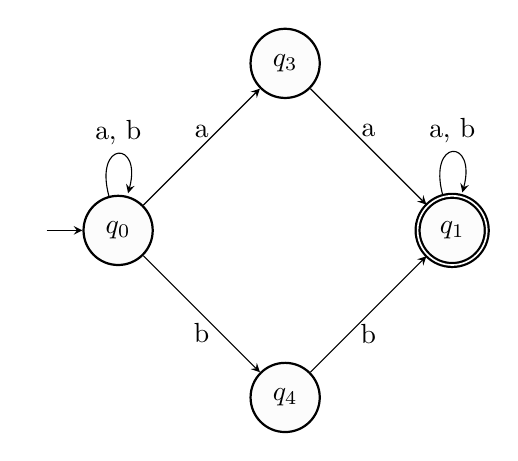
\begin{tikzpicture}
\node[state, initial] (q0) {$q_0$};
\node[state,above right of=q0] (q3) {$q_3$};

\node[state,  below right of=q0] (q4) {$q_4$};
\node[state, accepting, below right of=q3] (q1) {$q_1$};


\draw 

(q0) edge[loop above] node{a, b } (q0)
(q0) edge[left,above] node{a} (q3)
(q0) edge[left,below] node{b} (q4)
(q3) edge[left,above] node{a} (q1)
(q4) edge[left,below] node{b} (q1)
(q1) edge[loop above] node{a, b } (q1);


\end{tikzpicture}
%\caption*{Caption.}

\end{figure}
\end{frame}

\begin{frame}{Example 8.19}
%\textcolor{blue}{
	% Construct a TM for the regular expression $(a + b)^{*}(aa + bb)(a + b)^{*}$.}
	 
	 
	\textcolor{red}{Continue the solution:}Inserting a new initial state $q_{i}$
 and final state $q_{H}$, the finite automata becomes
 \begin{figure}[H] % ’ht’ tells LaTeX to place the figure ’here’ or at the top of the page
\centering % centers the figure
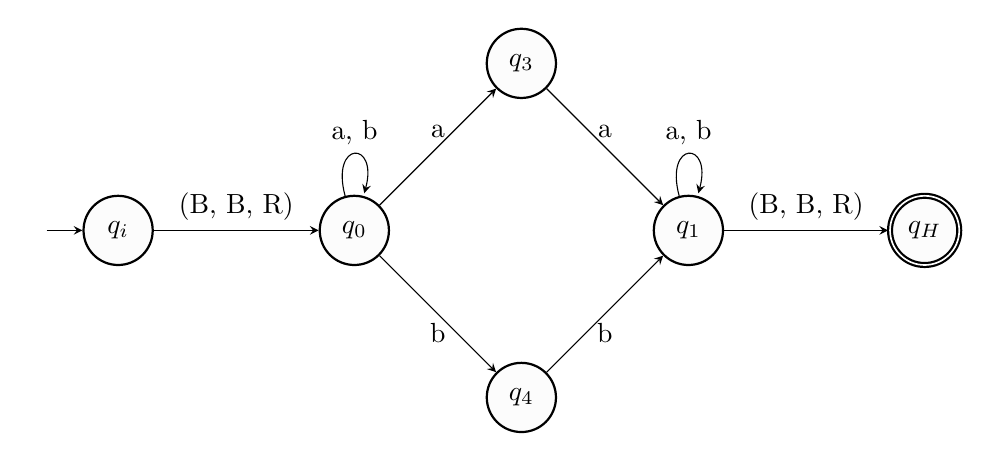
\begin{tikzpicture}
\node[state, initial] (qi) {$q_i$};
\node[state, right of=qi] (q0) {$q_0$};
\node[state,above right of=q0] (q3) {$q_3$};

\node[state,  below right of=q0] (q4) {$q_4$};
\node[state, below right of=q3] (q1) {$q_1$};
\node[state, accepting, right of=q1] (qH) {$q_H$};


\draw 
(qi) edge[right, above] node{(B, B, R) } (q0)
(q0) edge[loop above] node{a, b } (q0)
(q0) edge[right,above] node{a} (q3)
(q0) edge[right,below] node{b} (q4)
(q3) edge[right,above] node{a} (q1)
(q4) edge[right,below] node{b} (q1)
(q1) edge[loop above] node{a, b } (q1)
(q1) edge[right, above] node{(B, B, R) } (qH);

\end{tikzpicture}
%\caption*{Caption.}

\end{figure}
\end{frame}


\begin{frame}{Example 8.19}
%	\textcolor{blue}{ Construct a TM for the regular expression $(a + b)^{*}(aa + bb)(a + b)^{*}$.}
	 
 
\textcolor{red}{Continue the solution:} Converting the levels of the inputs, the TM becomes
\begin{figure}[H] % ’ht’ tells LaTeX to place the figure ’here’ or at the top of the page
\centering % centers the figure
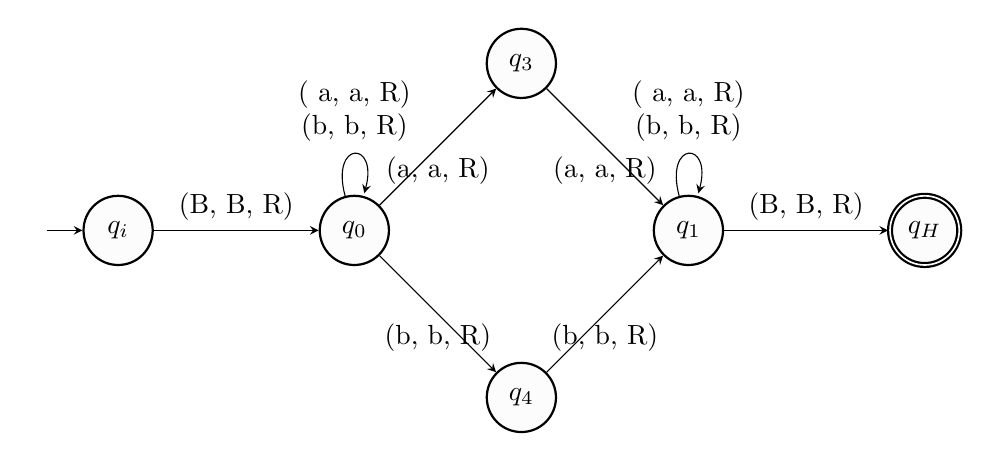
\begin{tikzpicture}
\node[state, initial] (qi) {$q_i$};
\node[state, right of=qi] (q0) {$q_0$};
\node[state,above right of=q0] (q3) {$q_3$};

\node[state,  below right of=q0] (q4) {$q_4$};
\node[state, below right of=q3] (q1) {$q_1$};
\node[state, accepting, right of=q1] (qH) {$q_H$};


\draw 
(qi) edge[right, above] node{(B, B, R) } (q0)
(q0) edge[loop above] node{\begin{tabular}{c} ( a, a, R) \\ (b, b, R)  \end{tabular}  } (q0)
(q0) edge[right,below] node{(a, a, R)} (q3)
(q0) edge[right,below] node{(b, b, R)} (q4)
(q3) edge[right,below] node{(a, a, R)} (q1)
(q4) edge[right,below] node{(b, b, R)} (q1)
(q1) edge[loop above] node{\begin{tabular}{c} ( a, a, R) \\ (b, b, R)  \end{tabular}} (q1)
(q1) edge[right, above] node{(B, B, R) } (qH);

\end{tikzpicture}
\end{figure}
\end{frame}


%\backupend

\end{document}
			
